\subsection{Verifica dell'indirizzo email}
\subsubsection{MustVerifyEmai}
Per la verifica dell'indirizzo email, il modello \verb|User| deve implementare il contatto \verb|Illuminate\Contracts\Auth\MustVerifyEmai|~\cite{LaravelEmailVerification}.
\subsubsection{Laravel Route}
Per implementare la verifica dell'indirizzo e-mail sono state definite due route nel file \verb|routes\api\auth.php| (Codice ~\ref{lst:route_verifica_email}).

La prima permette di gestire la verifica dell'indirizzo e-mail, mentre la seconda permette di inviare nuovamente una e-mail all'utente per la verifica del suo indirizzo email.
\begin{lstlisting}[caption={Route per la verifica dell'indirizzo e-mail}, label={lst:route_verifica_email}]
Route::get('email/verify/{id}/{hash}', [
	VerifyEmailController::class, '__invoke'
])->middleware(['auth:api', 'signed'])
	->name('verification.verify');

Route::post('email/verification-notification', [
	EmailVerificationNotificationController::class,
	'store'
])->middleware(['auth:api', 'throttle:6,1']);
\end{lstlisting}

\subsubsection{E-mail di verifica}
L'e-mail che verr\`a inviata all'utente viene definita attraverso una chiusura passata come parametro al metodo \verb|toMailUsing| della classe \verb|Illuminate\Auth\Notifications\VerifyEmail| nel metodo \verb|boot()| della classe \verb|App\Providers\AuthServiceProvider|. Tale chiusura \`e definita nel seguente modo:
\begin{lstlisting}[caption={E-mail di verifica}, label={lst:route_registration}]
VerifyEmail::toMailUsing(function ($notifiable, $url) {
	return (new MailMessage)
		->subject('Verify Email Address')
		->greeting('Welcome to atARTIST, ' . $notifiable->name)
		->line('Click the button below to verify your email address.')
		->action('Verify Email Address', $url);
});
\end{lstlisting}
e produce come risultato l'e-mail nella figura sottostante (Figura~\ref{fig:email_di_verifica}).
\begin{figure}[htbp]
	\centering
	\fboxsep=0.5pt
	\fboxrule=0.5pt
	\fcolorbox{black}{black}{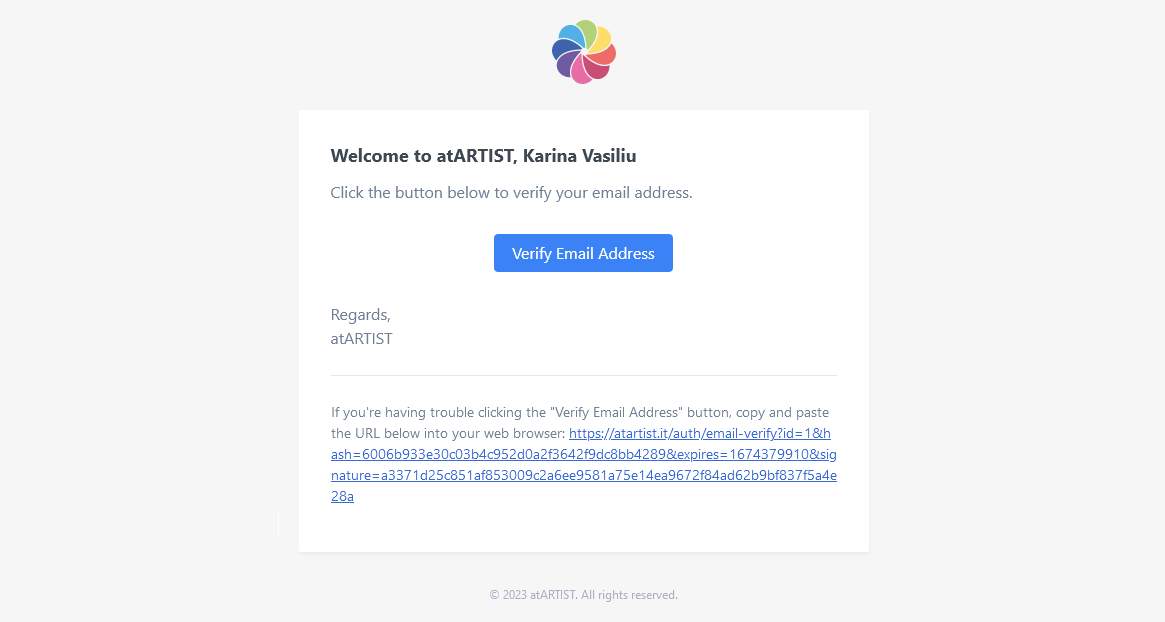
\includegraphics[width=0.8\linewidth]{figure/email}}
	\caption{E-mail per la conferma dell'indirizzo email}
	\label{fig:email_di_verifica}
\end{figure}


\subsubsection{Pagina di verifica}
Il link ricevuto via e-mail porta l'utente alla pagina ``auth/email-verify'' rappresentata dal componente Vue \verb|views/Auth/EmailVerify.vue|. Tale componente, una volta terminato il rendering iniziale, controlla che nell'URL siano presenti i parametri \verb|id|, \verb|hash|, \verb|expires| e \verb|signature|, i quali sono necessari per la verifica dell'indirizzo email. In tal caso esegue l'azione \verb|verifyEmail| dello store Pinia \verb|UserStore|. Tale azione invia una richiesta GET all'URI dell'API \verb|email/verify/{id}/{hash}| passando i parametri \verb|expires| e \verb|signature| dell'URL come parametri della richiesta.

Se la richiesta ha successo, l'azione \verb|verifyEmail| modifica l'oggetto \verb|user|, presente nello stato dello store, impostando come \verb|true| l'attributo \verb|verified_email| e l'utente viene reindirizzato alla homepage. Se invece la richiesta fallisce, l'utente viene reindirizzato alla pagina ``not-found''.
